%!TEX program = xelatex
\documentclass[a4paper,UTF8]{ctexart}

\usepackage{natbib}
\usepackage{graphicx}
\usepackage{enumitem}
\usepackage{float}
\usepackage[newfloat]{minted}
\usepackage[hidelinks]{hyperref}
\usepackage[labelfont=bf]{caption}
\usepackage{geometry}

\geometry{left=2cm, right=2cm, top=2cm, bottom=2cm}
\AtBeginDocument{%
	\renewcommand{\sectionautorefname}{章节\negthinspace}
	\renewcommand{\subsectionautorefname}{章节\negthinspace}
	\renewcommand{\subsubsectionautorefname}{章节\negthinspace}
	\renewcommand{\figureautorefname}{图\negthinspace}
	\renewcommand{\tableautorefname}{表\negthinspace}
}
\newenvironment{code}{\captionsetup{type=listing}}{}
\SetupFloatingEnvironment{listing}{name=代码}
\captionsetup[listing]{skip=-8pt}

\graphicspath{ {./img/} }

\usemintedstyle{tango}
\setminted{
	autogobble=true,
	frame=lines,
	framesep=1mm,
	fontsize=\small,
	baselinestretch=1.0,
	tabsize=4,
	obeytabs=false,
	breaklines
}

\begin{document}

\title{LSM-KV 项目报告}
\date{\today}
\maketitle

\section{背景介绍}
Log-Structured Merge-Tree\cite{o1996log}(即LSM树)是一种面向磁盘、分层存储的数据结构。该数据结构被运用于Bigtable\cite{chang2008bigtable}、LevelDB、RocksDB等NoSQL数据库中。
\par
对于一个典型的LSM树,其内存数据被称为MemTable,跳表是一种常用的MemTable实现方法;磁盘中的数据文件被称为SSTable,存储在不同的层级(Level)中。当某个层级的SSTable数量超过该层级限制,则触发Compaction将相邻层级中重叠的SSTable合并写入到下一层级,直到所有层级的SSTable数量满足限制。
\par
相比B树、B+树等传统的面向磁盘数据结构,LSM树的写入操作与顺序读取操作的延迟较小。其主要原因是:
\begin{itemize}
	\item LSM树在插入数据时无需像B树、B+树频繁通过磁盘IO更新索引信息,而是在MemTable或者某个层级已满时集中做磁盘操作,减少了磁盘IO系统调用的次数,提升了写入效率。
	\item LSM树的每个SSTable都按键值顺序存储数据,且LSM树的Compaction机制减少了SSTable的键值重叠,这使得键值相邻的数据有大概率处在同一个SSTable中,提高了顺序读取效率。
\end{itemize}
% 这部分应该写LSM-KV这个Project的背景知识和你对这个Project的一些初步理解。 下面是教你如何在 \LaTeX 中插入一张图片。

\section{代码实现}
本文中实现的LSM树使用C++17结合模板编写,能够灵活切换索引缓存方法、MemTable数据结构(默认为SkipList,支持其他数据结构)、Level配置、键值(Key)与值(Value)的类型、Value的IO方法(支持自定义序列化或压缩算法),且不引入额外的运行时开销。
\par
LSM树实现了Get、Put、Delete、Scan、Reset方法,其中Scan的实现运用了二叉堆。
\par
此外,代码实现中使用一个LRU Cache来缓存std::ifstream对象,显著减少了打开文件的系统调用开销。LRU Cache的大小在运行时指定。

\subsection{样例}
\autoref{lst:StandardKVDef}定义了一个项目指定的标准LSM树,该LSM树使用Murmur3作为Bloom Filter的哈希算法。\autoref{lst:CompressedKVDef}定义了一个使用Snappy压缩算法压缩Value的LSM树,且该LSM树不缓存键值。

\begin{code}
	\begin{minted}{c++}
#include <lsm/kv.hpp>
#include "MurmurHash3.h"

template <typename Key> struct Murmur3BloomHasher {
	template <std::size_t Bits, typename Array> inline static void Insert(Array &array, const Key &key) {
		uint32_t hashes[4];
		MurmurHash3_x64_128(&key, sizeof(Key), 1, hashes);
		array[hashes[0] % Bits] = true;
		array[hashes[1] % Bits] = true;
		array[hashes[2] % Bits] = true;
		array[hashes[3] % Bits] = true;
	}
	template <std::size_t Bits, typename Array> inline static bool Exist(const Array &array, const Key &key) {
		uint32_t hashes[4];
		MurmurHash3_x64_128(&key, sizeof(Key), 1, hashes);
		return array[hashes[0] % Bits] && array[hashes[1] % Bits] && array[hashes[2] % Bits] && array[hashes[3] % Bits];
	}
};

template <typename Key> struct StandardTrait : public lsm::KVDefaultTrait<Key, std::string> {
	using Compare = std::less<Key>;
	using Container = lsm::SkipList<Key, lsm::KVMemValue<std::string>, Compare, std::default_random_engine, 1, 2, 32>;
	using KeyFile = lsm::KVCachedBloomKeyFile<Key, StandardTrait, lsm::Bloom<Key, 10240 * 8, Murmur3BloomHasher<Key>>>;
	constexpr static lsm::size_type kMaxFileSize = 2 * 1024 * 1024;

	constexpr static lsm::KVLevelConfig kLevelConfigs[] = {
	    {2, lsm::KVLevelType::kTiering},
		{4, lsm::KVLevelType::kLeveling},
		{8, lsm::KVLevelType::kLeveling},
	    {16, lsm::KVLevelType::kLeveling},
		{32, lsm::KVLevelType::kLeveling}
	};
};

using StandardKV = lsm::KV<uint64_t, std::string, StandardTrait<uint64_t>>;
	\end{minted}
	\caption{项目指定的标准LSM树定义}
	\label{lst:StandardKVDef}
\end{code}

\begin{code}
	\begin{minted}{c++}
#include <lsm/kv.hpp>
#include <snappy.h>

struct SnappyStringIO {
	inline static lsm::size_type GetSize(const std::string &str) {
		std::string compressed;
		snappy::Compress(str.data(), str.length(), &compressed);
		return compressed.length();
	}
	template <typename Stream> inline static void Write(Stream &ostr, const std::string &str) {
		std::string compressed;
		snappy::Compress(str.data(), str.length(), &compressed);
		ostr.write(compressed.data(), compressed.length());
	}
	template <typename Stream> inline static std::string Read(Stream &istr, lsm::size_type length) {
		std::string compressed, str;
		compressed.resize(length);
		istr.read(compressed.data(), length);
		snappy::Uncompress(compressed.data(), length, &str);
		return str;
	}
};

template <typename Key> struct CompressedTrait : public lsm::KVDefaultTrait<Key, std::string> {
	using KeyFile = lsm::KVUncachedKeyFile<Key, CompressedTrait>;
	using ValueIO = SnappyStringIO;
};

using CompressedKV = lsm::KV<uint64_t, std::string, CompressedTrait<uint64_t>>;
	\end{minted}
	\caption{使用Snappy压缩算法且不缓存键值的LSM树定义}
	\label{lst:CompressedKVDef}
\end{code}


\section{性能测试}

% 此部分主要是展现你实现的项目的测试,主要分为下面几个子部分。测试部分应当是文字加上测试数据的图片展示。

\subsection{预期结果}

% 在给定下面几个测试的具体数据之前,你应当首先在本节在理论上分析这些测量的结果,此步无需定量,是定性分析,
% 如果此处的分析与后面的具体数据测试有出入,请你给出你理解的导致这种出入的可能性。

根据LSM树的性质,在Get、Put、Delete三种操作中,只有Put与Delete操作可能触发磁盘写入和Compaction;同时Get与Put涉及的磁盘IO数据量较大,Delete至多只需写入一个不带Value的Key。因此常规测试中的操作延迟从大到小应为Put、Get、Delete,吞吐量则相反。
\par
相比不缓存键值数据,理论上使用Bloom Filter能够在命中率较低时减少无效文件访问次数以降低Get延迟,但会增加高命中率时Get操作的延迟;索引缓存极大减少了Get操作的IO次数,Get操作的延迟相比不缓存索引理论上会极大减少;缓存Bloom Filter和索引理论上不会比仅缓存索引有太大效率提升,因为内存中的二分查找效率已经足够高。
\par
Put操作中Compaction的开销与当前SSTable的数量有关。SSTable数量占满的层数越多,则Compaction需要处理的平均层数越多,Put的吞吐量越低。
\par
Level配置对吞吐量的影响有两个方面。首先,Tiering层与较小的文件数目限制会减少SSTable的重叠,提升Get与Scan的吞吐量;然而这会增加Put操作中Compaction的频率,降低Put的吞吐量。

\subsection{常规分析}
% \begin{enumerate}
% 	\item 包括Get、Put、Delete操作的延迟,你需要测出不同数据大小时的操作延迟,为了测试的合理性,你应当对每个数据大小测量然后计算出平均延迟
% 	\item 包括Get、Put、Delete操作的吞吐,意思是指系统单位时间内能够相应的请求的次数,显然,在展示你测试的时候你需要指明Key、Value的大小(注意是数据的大小,并不是具体的值)
% \end{enumerate}
本文分别测试了2 KiB、4 KiB、6 KiB、8 KiB数据大小的Put、Get、Delete操作的延迟与吞吐量,其中对Get操作分别测试了顺序和乱序的延迟与吞吐量,测试结果见\autoref{fig:Latency}和\autoref{fig:Throughput}。

\begin{figure}[htbp]
	\centering
	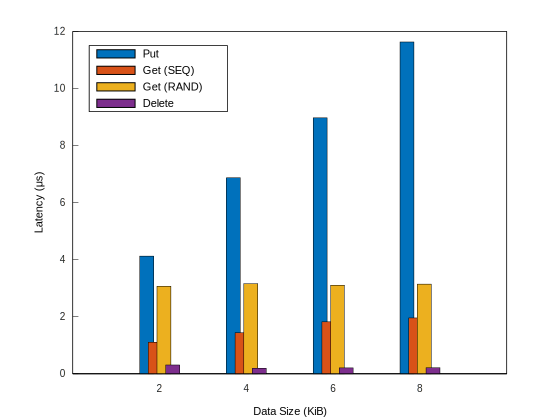
\includegraphics[width=.6\textwidth]{latency.pdf}
	\caption{标准LSM树在不同数据大小下Put、Get、Delete操作的平均延迟}
	\label{fig:Latency}
\end{figure}
\begin{figure}[htbp]
	\centering
	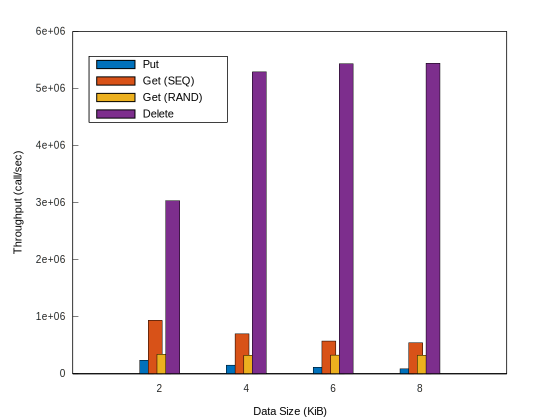
\includegraphics[width=.6\textwidth]{throughput.pdf}
	\caption{标准LSM树在不同数据大小下Put、Get、Delete操作的吞吐量}
	\label{fig:Throughput}
\end{figure}

\par
测试结果与预期结果一致。操作延迟从大到小为Put、Get、Delete,吞吐量则相反;且顺序Get操作的延迟小于乱序Get操作。
\par
此外,Put操作的延迟与数据大小基本呈现性关系,推测原因为数据越大,Compaction的频率越高,导致延迟增加。顺序Get操作的延迟也与数据大小正相关,推测原因是数据越大,读取时切换文件的频率越高。
\par
乱序Get与Delete操作的延迟与数据大小基本无关。对于乱序Get,这是由于乱序时切换文件的频率基本与数据大小无关;对于Delete,这是由于其写入数据量小且基本恒定。

\subsection{索引缓存与Bloom Filter的效果测试}
本文测试了不缓存、只使用Bloom Filter、只缓存索引、缓存索引+Bloom Filter四种情况下Get操作的平均延迟。总共进行了两组测试,命中率分别为100\%和50\%,其中50\%的命中率通过Put偶数键值并在连续键值区间内Get实现,测试结果见\autoref{fig:Cache100}和\autoref{fig:Cache50}。

\begin{figure}[htbp]
	\centering
	\includegraphics[width=.6\textwidth]{cache-100.pdf}
	\caption{不缓存、只使用Bloom Filter、只缓存索引、缓存索引和Bloom Filter的LSM树在2 KiB数据大小、100\%命中率下Get操作的平均延迟}
	\label{fig:Cache100}
\end{figure}
\begin{figure}[htbp]
	\centering
	\includegraphics[width=.6\textwidth]{cache-50.pdf}
	\caption{不缓存、只使用Bloom Filter、只缓存索引、缓存索引和Bloom Filter的LSM树在2 KiB数据大小、50\%命中率下Get操作的平均延迟}
	\label{fig:Cache50}
\end{figure}

\par
测试结果与预期基本一致。
\begin{itemize}
	\item 相比不缓存,使用Bloom Filter在命中率为50\%时降低了Get延迟,但在命中率为100\%时增加了延迟
	\item 缓存索引的Get延迟在任何情况远小于不缓存索引
	\item 缓存索引+Bloom Filter相比仅缓存索引Get延迟略微增大,因为Bloom Filter的计算量较大且不足以抵消节省的内存二分查找开销
\end{itemize}

\subsection{Compaction的影响}

本文测试了不断插入数据时Put操作的吞吐量变化。测试中每次Put插入的值大小为8 KiB,共执行16384次Put,总共插入128 MiB的值。由于数据方差过大,绘图前进行了窗口大小为2048的移动平均,实验结果见\autoref{fig:Compaction}。
\begin{figure}[htbp]
	\centering
	\includegraphics[width=.8\textwidth]{compaction.pdf}
	\caption{Put操作吞吐量随累计数据量的变化曲线}
	\label{fig:Compaction}
\end{figure}

\par
测试结果与预期基本一致。当没有触发Compaction机制时,Put操作吞吐量最大;随后第一层填满(约4 MiB的值),吞吐量骤降。在总插入大小低于20 MiB时,吞吐量的降低呈现阶梯状,之后则趋于稳定。这可以解释为填满标准LSM树的前几层时Compaction的文件合并次数增长速度较快,因此吞吐量阶梯状降低;随后由于Leveling层的键值范围不重叠,每次Compaction的文件合并次数基本维持稳定,于是吞吐量趋于稳定。

% 不断插入数据的情况下,统计每秒钟处理的PUT请求个数(即吞吐量),并绘制其随时间变化的折线图,测试需要表现出compaction对吞吐量的影响。可以让键值对中value占用的空间大一些,从而提高compaction的频率,这样效果比较明显

\subsection{Level配置的影响}

在LSM树的Compaction机制中,Tiering层在文件个数超出界限时需要将层级中所有文件与下一个层级合并,当Tiering层界限过大时,其开销远大于Leveling层。因此Tiering层通常在最上层且允许的文件数目最小,其他层级均为Leveling层。又由于LSM树在每相邻两个层级的最大文件数目比例相同时写入效率最高\cite{o1996log}。因此本文主要测试分析最上层的Tiering层级的允许文件数量TieringSize以及每相邻两个层级的最大文件数目比例SizeRatio对LSM树整体效率的影响。
\begin{figure}[htbp]
	\centering
	\includegraphics[width=.6\textwidth]{level-put.pdf}
	\caption{指定TieringSize和SizeRatio的LSM树Put操作的平均延迟}
	\label{fig:LevelPut}
\end{figure}
\par
测试中使用的层级数量为5的LSM树,分别在$[1, 5]$区间内调整TieringSize和SizeRatio,测试Put与顺序Get操作的平均延迟。测试中每次写入的数据大小为8 KiB,总共写入128 MiB的值。由于Delete操作的延迟显著低于Put与Get,对LSM树性能构成的影响有限,不进行测试。测试结果见\autoref{fig:LevelPut}、\autoref{fig:LevelGet}。
\begin{figure}[htbp]
	\centering
	\includegraphics[width=.6\textwidth]{level-get.pdf}
	\caption{指定TieringSize和SizeRatio的LSM树Get操作的平均延迟}
	\label{fig:LevelGet}
\end{figure}

\par
测试结果与预期部分一致。由\autoref{fig:LevelGet}可见,当TieringSize大于2时,Get操作延迟相比TieringSize小于2时显著减小;继续增大TieringSize对Get延迟的降低不显著。
\par
根据\autoref{fig:LevelPut},Put的延迟随着TieringSize的增大先增加后减小,这与预期结果由一定差别,可能的原因是当TieringSize较大时,每个层级的容量相应增大,抵消了合并较大的Tiering层的开销;同时Put的延迟与SizeRatio则呈现较强的负相关性,这可以解释为较大的SizeRatio增大了层级容量,减少了Compaction的频率。
\par
综合以上测试结果,可以得出结论:选择较大的SizeRatio并选择大于2的TieringSize能同时降低Put和Get操作的延迟,然而这样显然也会导致整个数据库的总存储大小膨胀。因此本文给出的指导建议为:在存储空间允许的范围内尽可能提升SizeRatio,同时设置大于2的TieringSize。

% Level配置的影响:每一层的最大文件数目,每一层是Leveling还是Tiering是可以配置的变量。请选择其中一个变量,测试其对键值存储系统的吞吐量或时延的影响,请给出你测试不同情况时使用的配置文件内容,并解释你的测试结果。最终,请对如何进行Level配置给出指导性建议。

\section{结论}
LSM-KV项目使用C++17结合模版实现了可定制的LSM树,并对其进行了性能测试。
\par
常规分析、缓存与Bloom Filter测试、研究Compaction影响的实验结果基本符合理论预期;Level配置实验的结果能够用理论解释,且可以对Level配置给出指导建议。
\par
总体而言,LSM-KV项目的代码实现与实验较为成功。
% 对 Project 的整体总结,包括对实验结果的评价。

\section{致谢}
本项目LSM树核心代码中的LRU Cache实现借鉴了https://github.com/lamerman/cpp-lru-cache,除此之外均为独立编写,没有借鉴任何开源项目、论坛、博客。
\par
本文的背景介绍部分参考了https://zhuanlan.zhihu.com/p/415799237。
\par
本文中缓存与Bloom Filter测试的思路受到了https://medium.com/swlh/log-structured-merge-trees-9c8e2bea89e8的启发。
% 在此部分中,你需要列出项目过程中所受到的帮助并进行致谢,包括但不限于从同学、朋友、开源项目、论坛、博客等处获得的启发和帮助。注意,此处不包括老师和助教。


\section{其他和建议}
我认为项目要求应当鼓励同学学习使用最现代的C++,而非限制在C++14。
\par
C++17相比C++14增加了filesystem、constexpr if、更方便的type traits、结构化绑定等特性。C++20进一步引进了更多现代特性,例如concept、span等。
\par
本项目使用C++17实现的是为了简化代码的编写、提升可读性与运行效率。这不代表本项目无法使用C++14实现,只是需要写更多没有思维价值的代码。
\par
C++的最新特性很可能会在同学们的未来工作中使用,课程应当支持同学自学、运用。
% 这部分不做强制要求,你可以列出 LSM-KV Project中遇到的种种困难、挑战、bug、以及吐槽。


\bibliography{references.bib}
\bibliographystyle{alpha}

\end{document}
